% !TeX root = ../Notizen.tex
\subsection*{a)}
\begin{figure}[h!]
	\centering
	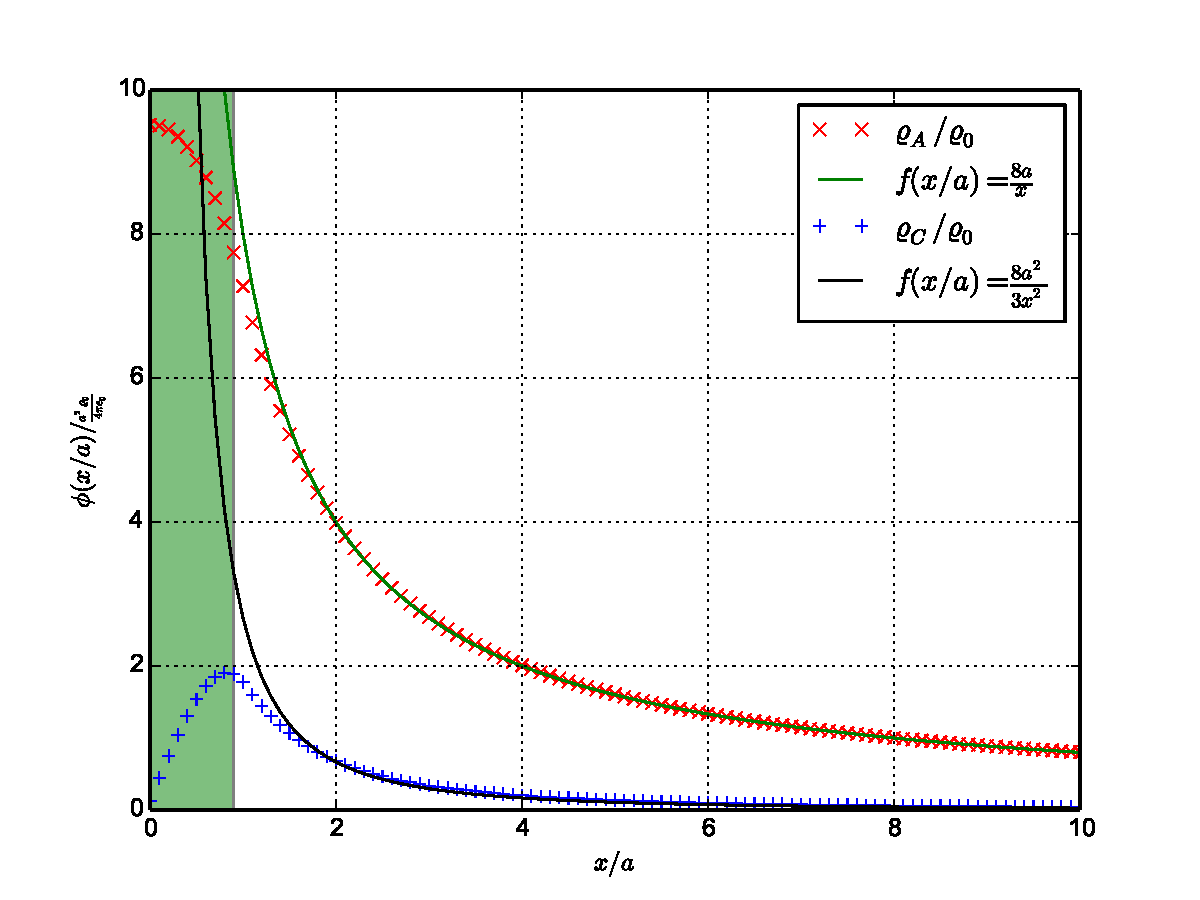
\includegraphics[width = \textwidth]{../Plots/Plot.pdf}
	\caption{\label{fig:Potentiale}Darstellung der Potentiale für den Bereich für $0<x/a<10$, sowie die dazugehörigen Asymptoten. Dabei ist in grün eingefärbt der Bereich innerhalb des Würfels.}
\end{figure}
Gegeben ist das Potential $\phi(x)$ mit
\begin{align}
	\phi(x)=\frac{1}{4\pi \epsilon_0}\int dx'\int dy' \int dz' \frac{\varrho(x' , y' ,z')}{\sqrt{(x-x')^2+(y')^2+(z')^2}}
\end{align}
wobei $x,\ y$ und $z$ die dreidimensionalen Raumkoordinaten darstellen und $\varrho$ die Ladungsdichte ist.
Hier wird die Ladungsdichte für einen gleichmäßig geladenen Würfel verwendet.
\begin{align}
 \varrho_A(x ,y ,z) = 
 \begin{cases}
 	\varrho_0, \text{ wenn } |x|<a,\ |y|<a,\text{ und } |z|<a\\
 	0,\text{\ \ \ sonst}
 \end{cases}
\end{align}
Um dies als Programm zu implementieren, werden die Koordinaten in Dimensionslose Koordinaten umgeschrieben.
\begin{align*}
	\tilde{x}=x/a\\
	\tilde{y}=y/a\\
	\tilde{z}=z/a\\
	\tilde{\varrho} = \varrho/\varrho_0
\end{align*}
Nach dieser Substitution folgt für das Potential
\begin{align}
	\phi(\tilde{x})=&\frac{\varrho_0 a^2}{4\pi \epsilon_0} \tilde{\phi }(\tilde{ x })\\
	\tilde{\phi}(\tilde{x})=&\int\limits_{-1}^{1}d\tilde{x}'\int\limits_{-1}^{1}d\tilde{y}'\int\limits_{-1}^{1}d\tilde{z}'
	\frac{1}{ \sqrt{\tilde{x} - \tilde{x}')^2 + (\tilde{y}')^2 + (\tilde{z}')^2} }
\end{align}
Die Ergebnisse für die Implementierung von $\phi(x)$ für $x\in[0,10]$ sind in \cref{fig:Potentiale} dargestellt.
Für die Asymptotik für große $x$, wird die Multipolentwicklung als Abschätzung verwendet:
\begin{align}
	\phi (\vec{r}) = \frac{1}{4\pi\epsilon_0}\left(\frac{Q}{r} + \frac{\vec{r}\vec{P}}{r^3}+\mathcal{O}(r^3)\right)
\end{align}
Wobei
\begin{align}
	Q=\int\varrho(\vec{r})d^3r\\
	\text{und}\\
	\vec{P}=\int \varrho(\vec{r})\vec{r}d^3r
\end{align}
definiert sind.
Der erste nicht verschwindende Term ist das Monopol $Q=\frac{8a^3}{4\pi\epsilon}$. Weshalb 
\begin{align}
 \tilde{\phi}(x) \propto \frac{8}{x}
\end{align}
für große $x$ abgeschätzt wird. Dies ist in \cref{fig:Potentiale} ebenfalls dargestellt.
\subsection*{b)}
Damit das Integral innerhalb des Würfels $(|x|<a,\ |y|<a$ und $|z|<a)$ keine Probleme bereiten, dadurch das durch Null geteilt wird, wird die Mittelpunktsregelverwendet. 
\subsection*{c)}
Hier wird nun ein inhomogen geladener Würfel betrachtet der durch
\begin{align}
	\varrho_C(x)=
	\begin{cases}
		\varrho_0\frac{x}{a}\text{ wenn } |x|<a,\ |y|<a \text{ und } |z|<a\\
		0,\text{\ \ \ \ sonst}
	\end{cases}
\end{align}
Für die Asymptotik wird wieder die Multipolentwicklung betrachtet.
Hier verschwindet allerdings der Monopol, weshalb als nächst höhere Ordnung der Duopol berechnet wird.
\begin{align}
	\vec{P} = \int\varrho(\vec{r})\vec{r}d^3r=\frac{8a^4\varrho_0}{3}\vec{e}_x
\end{align}
Daraus kann $\phi(x)$ als
\begin{align}
	\phi(x)\propto \frac{8}{3x^2}
\end{align}
abgeschätzt werden.
Das Potential sowohl durch numerische Berechnung, als auch durch Abschätzung, ist in \cref{fig:Potentiale} dargestellt.